\documentclass[crop,tikz]{standalone}


\usetikzlibrary{decorations.pathreplacing}
\usetikzlibrary{arrows}
\begin{document}
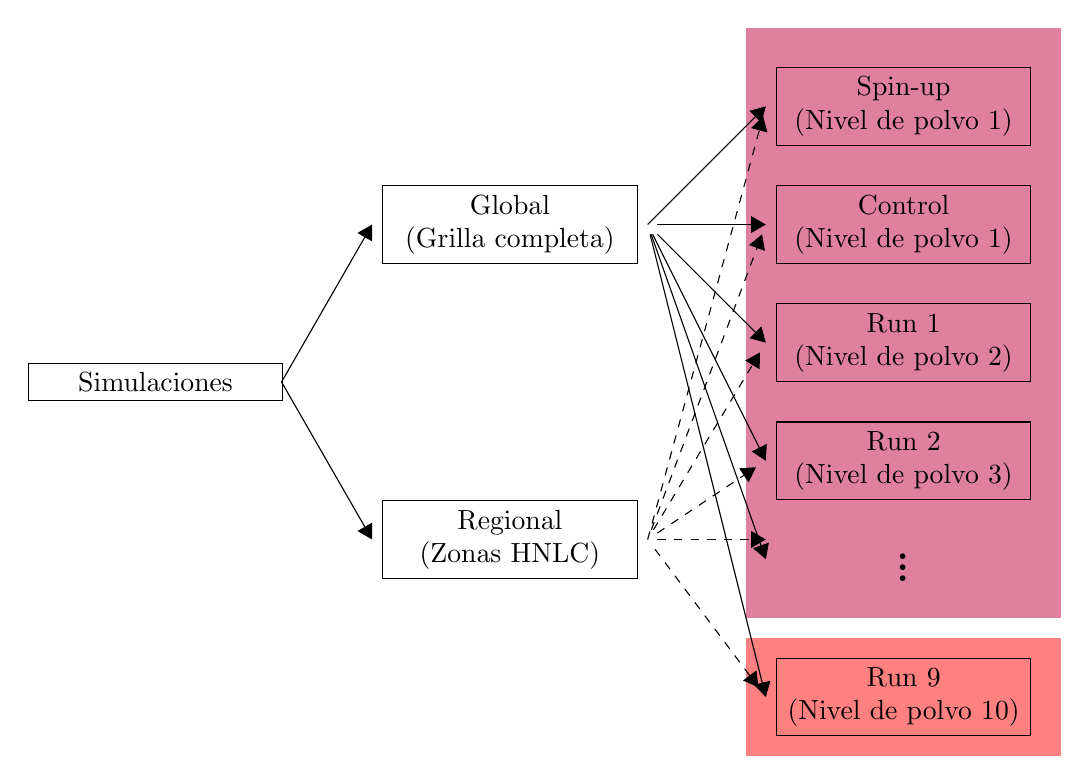
\begin{tikzpicture}
\tikzstyle{nodo texto}=[draw,text width= 3cm,align=center]


\node[nodo texto] at (-4.5,0) {Simulaciones };
\node[nodo texto] at (0,2) {Global \\ (Grilla completa)};
\node[nodo texto] at (0,-2) {Regional \\ (Zonas HNLC)};

\draw[draw=none,fill=purple!50]  (3,4.5) rectangle (7,-3);
\draw[draw=none,fill=red!50] (7,-3.25) rectangle (3,-4.75);

\node[nodo texto] at (5,3.5) {Spin-up \\ (Nivel de polvo 1)};
\node[nodo texto] at (5,2) {Control \\ (Nivel de polvo 1)};
\node[nodo texto] at (5,0.5) {Run 1 \\ (Nivel de polvo 2)};
\node[nodo texto] at (5,-1) {Run 2 \\ (Nivel de polvo 3)};
\node[nodo texto] at (5,-4) {Run 9 \\ (Nivel de polvo 10)};


\node[font=\Huge, sloped] at (5,-2.25) {$\vdots$};

\draw [-triangle 60](1.75,2) node (v1) {} -- (3.25,3.5) node (v2) {};
\draw [-triangle 60](v1) -- (3.25,2) node (v4) {};
\draw [-triangle 60](v1) -- (3.25,0.5) node (v5) {};
\draw [-triangle 60](v1) -- (3.25,-1) node (v6) {};
\draw [-triangle 60](v1) -- (3.25,-2.25);
\draw [-triangle 60](v1) -- (3.25,-4) node (v7) {};
\draw [dashed,-triangle 60](1.75,-2) node (v3) {} -- (v2);
\draw [dashed,-triangle 60](v3) -- (v4);
\draw [dashed,-triangle 60](v3) -- (v5);
\draw [dashed,-triangle 60](v3) -- (v6);
\draw [dashed,-triangle 60](v3) -- (3.25,-2);
\draw [dashed,-triangle 60](v3) -- (v7);
\draw [-triangle 60](-2.9,0) -- (-1.75,2);
\draw [-triangle 60](-2.9,0) -- (-1.75,-2);
\end{tikzpicture}
\end{document}
    